% ARTICLE 2 ----
% This is just here so I know exactly what I'm looking at in Rstudio when messing with stuff.
% Options for packages loaded elsewhere
\PassOptionsToPackage{unicode}{hyperref}
\PassOptionsToPackage{hyphens}{url}
%
\documentclass[
  11pt,
]{article}
\usepackage{lmodern}
\usepackage{amssymb,amsmath}
\usepackage{ifxetex,ifluatex}
\ifnum 0\ifxetex 1\fi\ifluatex 1\fi=0 % if pdftex
  \usepackage[T1]{fontenc}
  \usepackage[utf8]{inputenc}
  \usepackage{textcomp} % provide euro and other symbols
\else % if luatex or xetex
  \usepackage{unicode-math}
  \defaultfontfeatures{Scale=MatchLowercase}
  \defaultfontfeatures[\rmfamily]{Ligatures=TeX,Scale=1}
\fi
% Use upquote if available, for straight quotes in verbatim environments
\IfFileExists{upquote.sty}{\usepackage{upquote}}{}
\IfFileExists{microtype.sty}{% use microtype if available
  \usepackage[]{microtype}
  \UseMicrotypeSet[protrusion]{basicmath} % disable protrusion for tt fonts
}{}
\makeatletter
\@ifundefined{KOMAClassName}{% if non-KOMA class
  \IfFileExists{parskip.sty}{%
    \usepackage{parskip}
  }{% else
    \setlength{\parindent}{0pt}
    \setlength{\parskip}{6pt plus 2pt minus 1pt}
    }
}{% if KOMA class
  \KOMAoptions{parskip=half}}
\makeatother
\usepackage{xcolor}
\IfFileExists{xurl.sty}{\usepackage{xurl}}{} % add URL line breaks if available
\urlstyle{same} % disable monospaced font for URLs
\usepackage[margin=1in]{geometry}
\usepackage{longtable,booktabs}
% Correct order of tables after \paragraph or \subparagraph
\usepackage{etoolbox}
\makeatletter
\patchcmd\longtable{\par}{\if@noskipsec\mbox{}\fi\par}{}{}
\makeatother
% Allow footnotes in longtable head/foot
\IfFileExists{footnotehyper.sty}{\usepackage{footnotehyper}}{\usepackage{footnote}}
\makesavenoteenv{longtable}
\usepackage{graphicx}
\makeatletter
\def\maxwidth{\ifdim\Gin@nat@width>\linewidth\linewidth\else\Gin@nat@width\fi}
\def\maxheight{\ifdim\Gin@nat@height>\textheight\textheight\else\Gin@nat@height\fi}
\makeatother
% Scale images if necessary, so that they will not overflow the page
% margins by default, and it is still possible to overwrite the defaults
% using explicit options in \includegraphics[width, height, ...]{}
\setkeys{Gin}{width=\maxwidth,height=\maxheight,keepaspectratio}
% Set default figure placement to htbp
\makeatletter
\def\fps@figure{htbp}
\makeatother
\setlength{\emergencystretch}{3em} % prevent overfull lines
\providecommand{\tightlist}{%
  \setlength{\itemsep}{0pt}\setlength{\parskip}{0pt}}
\setcounter{secnumdepth}{5}

\ifluatex
  \usepackage{selnolig}  % disable illegal ligatures
\fi
\newlength{\cslhangindent}
\setlength{\cslhangindent}{1.5em}
\newlength{\csllabelwidth}
\setlength{\csllabelwidth}{3em}
\newenvironment{CSLReferences}[2] % #1 hanging-ident, #2 entry spacing
 {% don't indent paragraphs
  \setlength{\parindent}{0pt}
  % turn on hanging indent if param 1 is 1
  \ifodd #1 \everypar{\setlength{\hangindent}{\cslhangindent}}\ignorespaces\fi
  % set entry spacing
  \ifnum #2 > 0
  \setlength{\parskip}{#2\baselineskip}
  \fi
 }%
 {}
\usepackage{calc}
\newcommand{\CSLBlock}[1]{#1\hfill\break}
\newcommand{\CSLLeftMargin}[1]{\parbox[t]{\csllabelwidth}{#1}}
\newcommand{\CSLRightInline}[1]{\parbox[t]{\linewidth - \csllabelwidth}{#1}\break}
\newcommand{\CSLIndent}[1]{\hspace{\cslhangindent}#1}


\title{APPENDIX: Disagreement and dissent on a bench: a quantitative
empirical analysis of the Czech Constitutional Court}
\author{true \and true}
\date{October 12, 2023}

% Jesus, okay, everything above this comment is default Pandoc LaTeX template. -----
% ----------------------------------------------------------------------------------
% I think I had assumed beamer and LaTex were somehow different templates.


\usepackage{kantlipsum}

\usepackage{abstract}
\renewcommand{\abstractname}{}    % clear the title
\renewcommand{\absnamepos}{empty} % originally center

\renewenvironment{abstract}
 {{%
    \setlength{\leftmargin}{0mm}
    \setlength{\rightmargin}{\leftmargin}%
  }%
  \relax}
 {\endlist}

\makeatletter
\def\@maketitle{%
  \newpage
%  \null
%  \vskip 2em%
%  \begin{center}%
  \let \footnote \thanks
      {\fontsize{18}{20}\selectfont\raggedright  \setlength{\parindent}{0pt} \@title \par}
    }
%\fi
\makeatother


\title{APPENDIX: Disagreement and dissent on a bench: a quantitative
empirical analysis of the Czech Constitutional Court }

\date{}

\usepackage{titlesec}

% 
\titleformat*{\section}{\large\bfseries}
\titleformat*{\subsection}{\normalsize\itshape} % \small\uppercase
\titleformat*{\subsubsection}{\normalsize\itshape}
\titleformat*{\paragraph}{\normalsize\itshape}
\titleformat*{\subparagraph}{\normalsize\itshape}

% add some other packages ----------

% \usepackage{multicol}
% This should regulate where figures float
% See: https://tex.stackexchange.com/questions/2275/keeping-tables-figures-close-to-where-they-are-mentioned
\usepackage[section]{placeins}



\makeatletter
\@ifpackageloaded{hyperref}{}{%
\ifxetex
  \PassOptionsToPackage{hyphens}{url}\usepackage[setpagesize=false, % page size defined by xetex
              unicode=false, % unicode breaks when used with xetex
              xetex]{hyperref}
\else
  \PassOptionsToPackage{hyphens}{url}\usepackage[draft,unicode=true]{hyperref}
\fi
}

\@ifpackageloaded{color}{
    \PassOptionsToPackage{usenames,dvipsnames}{color}
}{%
    \usepackage[usenames,dvipsnames]{color}
}
\makeatother
\hypersetup{breaklinks=true,
            bookmarks=true,
            pdfauthor={Author 1 () and Author 2 ()},
             pdfkeywords = {},
            pdftitle={APPENDIX: Disagreement and dissent on a bench: a
quantitative empirical analysis of the Czech Constitutional Court},
            colorlinks=true,
            citecolor=blue,
            urlcolor=blue,
            linkcolor=magenta,
            pdfborder={0 0 0}}
\urlstyle{same}  % don't use monospace font for urls

% Add an option for endnotes. -----



% This will better treat References as a section when using natbib
% https://tex.stackexchange.com/questions/49962/bibliography-title-fontsize-problem-with-bibtex-and-the-natbib-package

% set default figure placement to htbp
\makeatletter
\def\fps@figure{htbp}
\makeatother



\usepackage{longtable}
\LTcapwidth=.95\textwidth
\linespread{1.05}
\usepackage{hyperref}
\usepackage{float}

\newtheorem{hypothesis}{Hypothesis}

\usepackage{setspace}

% trick for moving figures to back of document
% really wish we'd knock this shit off with moving tables/figures to back of document
% but, alas...

% 
% Optional code chunks ------
% SOURCE: https://stackoverflow.com/questions/50702942/does-rmarkdown-allow-captions-and-references-for-code-chunks



\begin{document}

% \textsf{\textbf{This is sans-serif bold text.}}
% \textbf{\textsf{This is bold sans-serif text.}}


% \maketitle

{% \usefont{T1}{pnc}{m}{n}
\setlength{\parindent}{0pt}
\thispagestyle{plain}
{%\fontsize{18}{20}\selectfont\raggedright
\maketitle  % title \par

}




{
   \vskip 13.5pt\relax \normalsize\fontsize{11}{12}
   \MakeUppercase{Author
1}, \small{}   \par \vskip -3.5pt \MakeUppercase{Author 2}, \small{}   

}

}






\vskip -8.5pt


 % removetitleabstract


\setlength{\parindent}{16pt}
\setlength{\parskip}{0pt}

% We'll put doublespacing here
\doublespacing
% Remember to cut it out later before bib
\vspace{30pt}

In this appendix, we explain our methodological choice of utilizing
Bayesian statistics, compare the performance of our machine learning
algorithm, and we diagnose and compare the models from our main article
and explain our research choices in finer detail.

\hypertarget{bayesian-framework}{%
\section{Bayesian framework}\label{bayesian-framework}}

Without delving too much into the Bayesian versus frequentist
statistics, we opt for the Bayesian framework for it, we believe,
reflects better our understanding of probability and scientific inquiry.
There are two major differences in understanding of concepts between the
two approaches towards statistics: that of role of prior knowledge and
that of probability.

In the frequentist framework, prior knowledge does not play too much of
a role and the inference is shaped solely by the observed data, whereas
in the Bayesian framework prior knowledge is updated with new data to
form new posterior conclusions. In other words, the Bayesian
statistician concerns themselves not with the uncertainty of the data
but also with how it fits into his prior knowledge.

That is reflected in different understandings of probability. The
frequentist understanding of probability refers to the long-run relative
frequency of a repeatable event. In other words, the main concern of
frequentist statistics is what would the frequency of any event be if we
could repeat it as many times as possible. The Bayesian probability
measures the relative plausibility of an event.

Science in general is based on the frequentist framework. The typical
quantitative studies are driven by finding a low enough p-value, i.e.,
the measure of probability of having observed data as or more extreme
than the observed data if in fact the original null hypothesis is
incorrect. In simple terms, the search for statistical significance is a
search for data so unlikely to have occurred due to chance, even if we
could gather them again and again.

The Bayesian framework rather than measuring the uncertainty about
observed data measures the uncertainty of the parameters of interests,
given the observed data and our prior knowledge. In simple terms, the
Bayesian statistician puts into doubt their conclusions about parameters
of a certain model, given the observed data and their prior knowledge.
Mathematically, the uncertainty is reflected in the fact that the
posterior parameters are drawn from a posterior distribution of the
model and are just an approximation of thereof in the form of
probability density function rather than a single value. The posterior
distribution of a parameter comes from simulating in our case 40000 (4
chains*10000 simulations) possible posterior models via the Monte Carlo
Markov Chain simulations.

\hypertarget{model-specifications-and-diagnoses}{%
\section{Model specifications and
diagnoses}\label{model-specifications-and-diagnoses}}

\hypertarget{model-1-classification-performance}{%
\subsection{Model 1 classification
performance}\label{model-1-classification-performance}}

To access the length of the majority argumentation, we needed to train a
classification algorithm that would automatically classify the over
90000 CCC decisions into their structural components, including the
court argumentation. We opted for a supervised machine learning
algorithm as performing such a task by hand was impossible.

Therefore, we manually annotated 200 randomly sampled decisions of the
CCC on the paragraph level. The categories that were to be classified by
the trained model: (1) heading, (2) verdict, (3) procedure history, (4)
complainant arguments, (5) court arguments, (6) conclusion, (7)
information on further legal remedies, (8) signature, and (9) dissenting
opinion.

We tested different classification algorithms and different ways to
represent the text. Following an unpublished Lüders paper (Lüders and
Stohlman 2023), we tested both the bag-of-words approach, in the form of
td-idf vectors, and dense word2vec vectors. In both cases, the basis for
the representation was the lemmatized text using the package UDPipe as
we found out that the lemmatization increased accuracy considerably in
either case.

It very quickly became clear that the dense word2vec vectors yielded
superior results, thus, we quickly abandoned the tf-idf representation
of text.\footnote{In comparison to the Lüders paper, who got reasonable
  results with the bag-of-words approach. Our assumption is that it is
  due to the fact that they tried to classify paragraphs based mostly on
  a presence of the word `proportionality'} Shortly put, we represented
the paragraphs as dense 300-dimensional vectors based on a pre-trained
word2vec model (Mikolov et al. 2013) on the whole text corpus of the
CCC, which we then recalculated for the whole paragraphs using doc2vec.
To the dense vectors, we added a very simple positional encoding in the
form of three additional features: the relative start position, end
position and length of the paragraph within the decision as whole
following previous research Eliášek, Kól, and Švaňa (2020){]}.

We tried a variety of common classifying algorithms: support vector
machines, XGBoost and random forests. The whole classification was
implemented using the tidymodels framework in R.

Because the positional encoding caused the issue of differing meanings
for the position between decisions with a dissenting opinion and
without\footnote{for example, in those without a dissenting opinion, the
  decision would typically end with court argumentation followed by
  signature, whereas in those with a dissenting opinion, the dissenting
  opinion was always at the end of the decision}, we ran our
classification in two steps. In the first step, a binary classification
model was trained only on the decisions including a dissenting opinion
to classify dissenting opinion paragraphs and the rest. The positional
encoding was then recalculated and a second classification model was
trained that classified the rest of the structure. The ensuing
prediction on previously unseen unannotated followed in the same two
steps.

We now present overview of the performance of the machine learning
algorithms. All the results are based only on the dense vector
representations, as we scraped the tf-idf early on in the process. The
tuning and testing process was done using a 10-fold cross-validation.
The training dataset was balanced out using SMOTE oversampling, because
the classes were heavily imbalanced. The XGBoost algorithm came out as
the most appropriate for the first step model with the highest accuracy
(and other metrics too, including the area under ROC curve, precision
etc.). The following table includes the top 5 performing algorithms with
differently tuned parameters.

\begin{longtable}[]{@{}lrr@{}}
\caption{Comparison of the performance of the first-step
algorithms}\tabularnewline
\toprule\noalign{}
model & accuracy & rank \\
\midrule\noalign{}
\endfirsthead
\toprule\noalign{}
model & accuracy & rank \\
\midrule\noalign{}
\endhead
\bottomrule\noalign{}
\endlastfoot
boost\_tree & 0.938 & 1 \\
rand\_forest & 0.918 & 2 \\
rand\_forest & 0.916 & 3 \\
rand\_forest & 0.917 & 4 \\
svm\_linear & 0.905 & 5 \\
\end{longtable}

The final fitted model yielded the following metrics. The precision is
satisfactory for our purposes as here we were interested mainly in
separating dissents from the rest. The zero rule for our dataset is
0.77, the proportion of our majority class, i.e., our precision of 0.86
is well above the zero rule.

\begin{longtable}[]{@{}lr@{}}
\caption{Performance of the final first-step fit XGBoost
algorithm}\tabularnewline
\toprule\noalign{}
metric & value \\
\midrule\noalign{}
\endfirsthead
\toprule\noalign{}
metric & value \\
\midrule\noalign{}
\endhead
\bottomrule\noalign{}
\endlastfoot
accuracy & 0.936 \\
recall & 0.858 \\
f\_meas & 0.859 \\
precision & 0.860 \\
mcc & 0.818 \\
roc\_auc & 0.981 \\
\end{longtable}

In the second step, we recalculated the positional encoding of the
decisions by separating the dissenting opinion from the rest of the
decision so that the structure now resembled the decisions without a
dissenting opinion. We again tested multiple classification algorithms,
with the XGBoost coming out on top.

\begin{longtable}[]{@{}lrr@{}}
\caption{Comparison of the performance of the second-step
algorithms}\tabularnewline
\toprule\noalign{}
model & precision & rank \\
\midrule\noalign{}
\endfirsthead
\toprule\noalign{}
model & precision & rank \\
\midrule\noalign{}
\endhead
\bottomrule\noalign{}
\endlastfoot
boost\_tree & 0.805 & 1 \\
boost\_tree & 0.812 & 2 \\
rand\_forest & 0.808 & 3 \\
svm\_linear & 0.766 & 4 \\
svm\_linear & 0.767 & 5 \\
svm\_linear & 0.768 & 6 \\
\end{longtable}

The resulting metrics are reasonably good, the zero rule lays at 0.38,
thus, our trained model greatly outperforms the zero rule.

\begin{longtable}[]{@{}lr@{}}
\caption{Performance of the final second-step fit XGBoost
algorithm}\tabularnewline
\toprule\noalign{}
metric & value \\
\midrule\noalign{}
\endfirsthead
\toprule\noalign{}
metric & value \\
\midrule\noalign{}
\endhead
\bottomrule\noalign{}
\endlastfoot
accuracy & 0.821 \\
recall & 0.843 \\
f\_meas & 0.824 \\
precision & 0.815 \\
mcc & 0.749 \\
roc\_auc & 0.979 \\
\end{longtable}

\hypertarget{model-1-diagnosis}{%
\subsection{Model 1 diagnosis}\label{model-1-diagnosis}}

Our first model concerns the length of the decision, with the outcome
variable of interest being a discrete count of words. At first glance,
we assumed that

\[
Y_{words} | \lambda \sim Pois(\lambda)
\]

because our outcome variable of interest is a discrete count and the
density plot (Fig. 1) of the length of court argumentation suggests so.

\vspace{25pt}

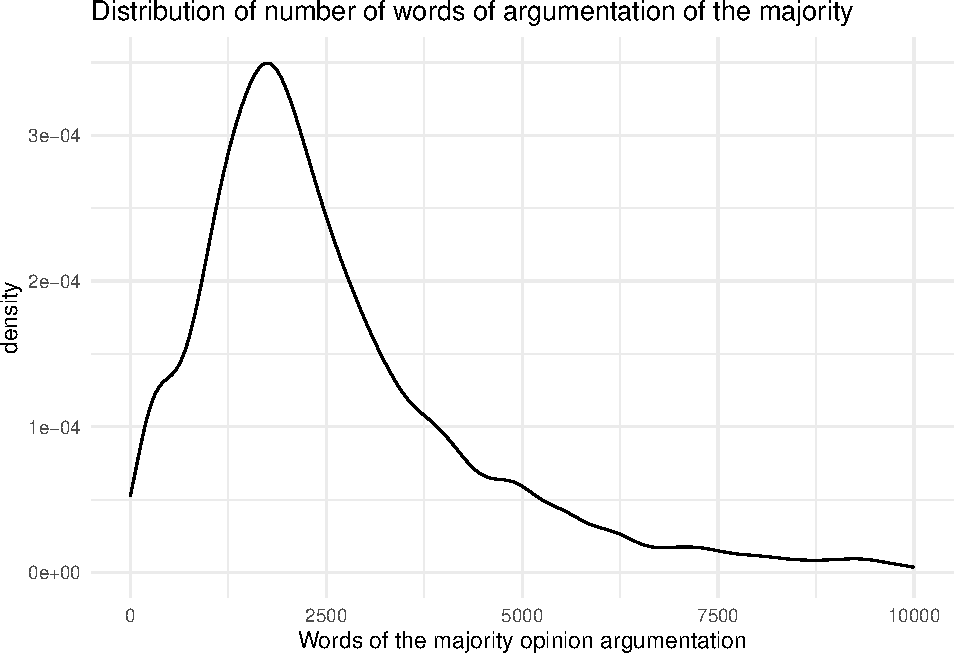
\includegraphics{dissents_article_appendix_files/figure-latex/negbinom-1.pdf}
\vspace{25pt}

However, as the posterior checking revealed, the Y was actually
overdispersed and the Poisson regression was not able to capture the
overdispersion. Therefore, we instead opted for the Negative Binomial
model, which allows for relaxing the assumption of equality of variance
of Y to its expected value. Thus, the explanatory variable, the number
of words of argumentation of the CCC \emph{Y}

\[
Y_{words} | \mu, r \sim NegBin(\mu, r)
\]

We opted for a completely pooled model as the data did not contain any
inherent structure (there were no clusters). As for the priors, we based
the priors on the cursory exploratory peak into the data. All our priors
follow a normal distribution, the intercept being centered around the
population mean. The remaining priors were kept uninformative via the
autoscale = TRUE argument, because we simply have no previous knowledge
about the CCC.

We ran the model via Stan with 4 Monte Carlo Markov Chains (MCMC) of
20000 iterations each, the first 10000 warm up iterations being
discarded. The trace plot shows that the chains were stable and probed
plausible parameter values, the density plots of the MCMC show that all
4 chains exhibited similar behavior, and the autocorrelation between the
iterations always dropped quickly and that the chains were moving around
the potential parameter values quickly (Fig. 2).

\vspace{25pt}

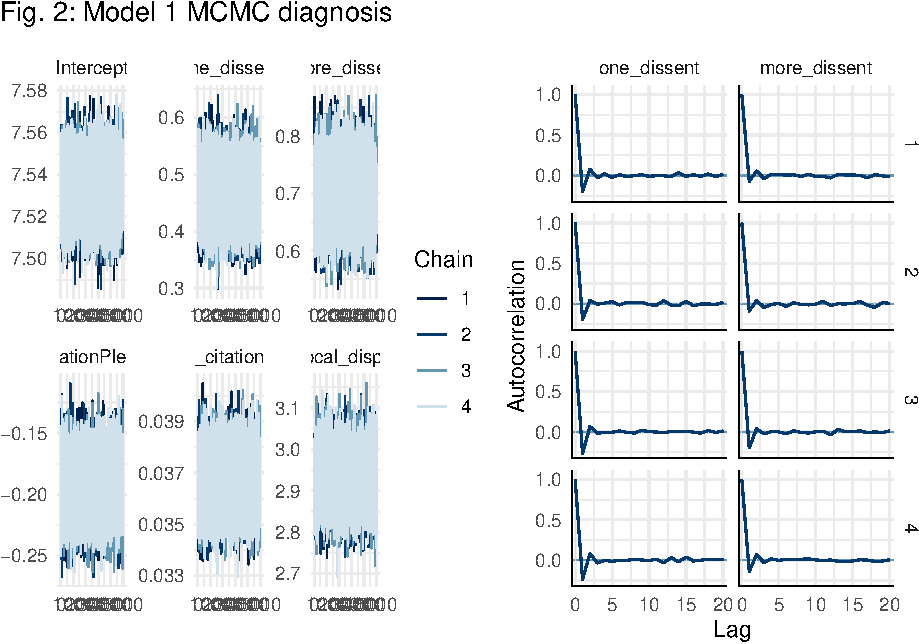
\includegraphics{dissents_article_appendix_files/figure-latex/model1_diagnosis-1.pdf}
\vspace{25pt}

The posterior predictive check (Fig. 3) confirms that although the
simulations are not perfect, they do reasonably capture the features of
the observed number of words of court arguments. In other words, we
selected the correct model and the priors are not too off either. Thus,
our Negative Binomial regression assumptions are reasonable.

\vspace{25pt}

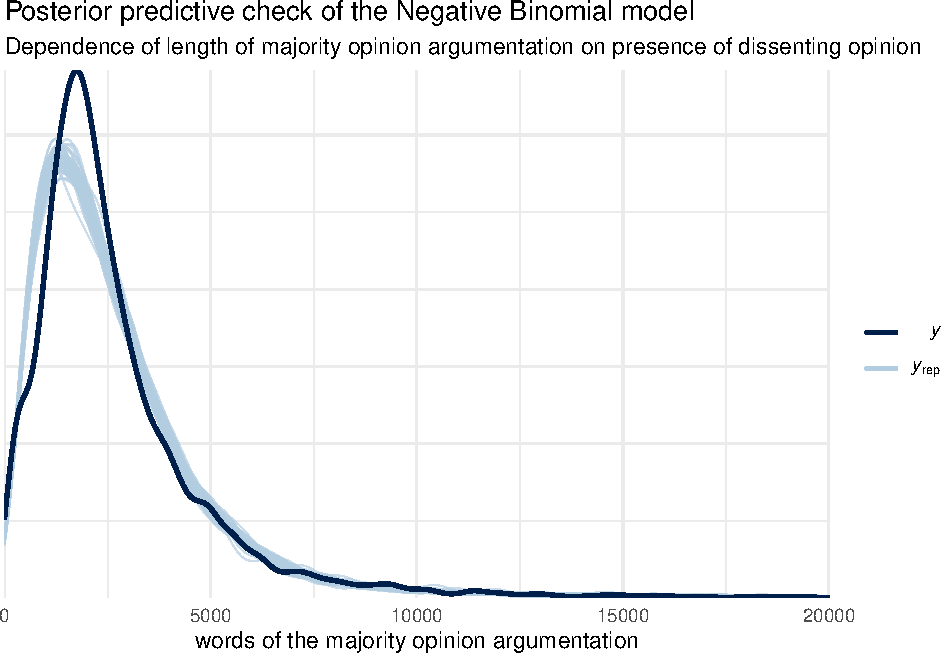
\includegraphics{dissents_article_appendix_files/figure-latex/pp_check_negbinom-1.pdf}
\vspace{25pt} The model got the median posterior prediction 0.57
standard deviations off the observed Y with 93 \% of the observed Y
values falling within the 95 \% posterior credible interval. It is also
clear that the negative binomial model yields far more accurate results
than the poisson (compare the scaled MAE). 10-fold cross-validated
posterior check reveals the model did not overfit.

\begin{longtable}[]{@{}lrrrr@{}}
\caption{Posterior prediction summaries of performance of Model
1}\tabularnewline
\toprule\noalign{}
model & mae & mae\_scaled & within\_50 & within\_95 \\
\midrule\noalign{}
\endfirsthead
\toprule\noalign{}
model & mae & mae\_scaled & within\_50 & within\_95 \\
\midrule\noalign{}
\endhead
\bottomrule\noalign{}
\endlastfoot
poisson & 893.70 & 17.79 & 0.02 & 0.05 \\
neg\_bin & 802.68 & 0.57 & 0.57 & 0.93 \\
\end{longtable}

\hypertarget{model-2-diagnosis}{%
\subsection{Model 2 diagnosis}\label{model-2-diagnosis}}

Our second model features a binomial variable as the outcome variable of
interest. Thus, we opt for a Bayesian logistic regression.

We tried two models, a completely pooled and hierarchical model
clustered around the judges. The main difference between the two models
is that the former model completely ignores individual intercept. The
latter allows for differentiating intercepts between the groups (in our
case the individual judges) and the global intercept. The global
parameter of interest is then informed both by the global trends as well
as the individual intercepts. That can usually lead to higher accuracy
in case of structured or time series data at the cost of higher
computational expenses.

We ran both the models via Stan with 4 Monte Carlo Markov Chains (MCMC)
of 20000 iterations each, the first 10000 warm up iterations being
discarded. We did a diagnosis of all the models. In both cases, the
trace plots show that the chains were stable and probed plausible
parameter values, the density plots of the MCMC show that all 4 chains
exhibited similar behavior, and the autocorrelation between the
iterations always dropped quickly and that the chains were moving around
the potential parameter values quickly (Fig. 4).

\vspace{25pt}

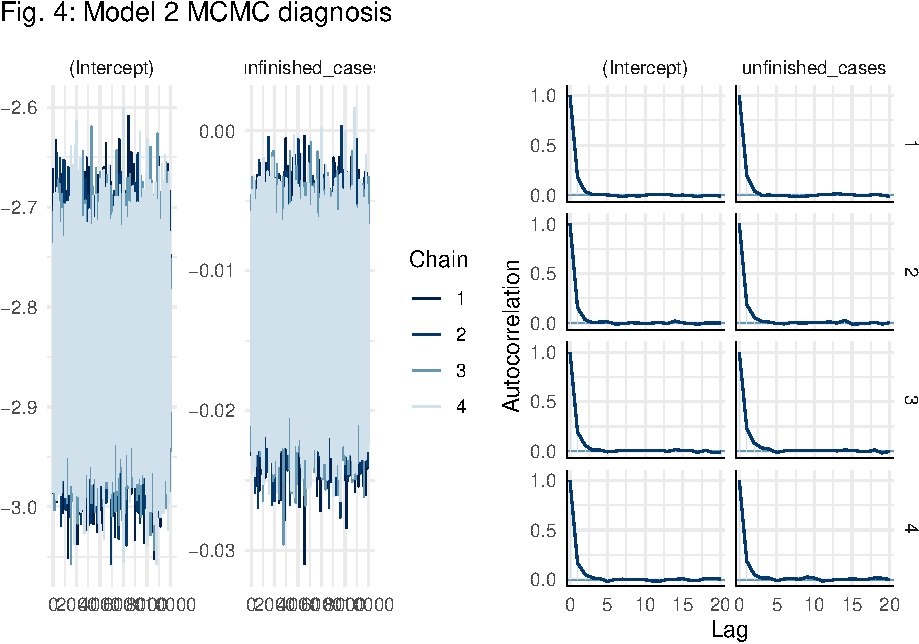
\includegraphics{dissents_article_appendix_files/figure-latex/mcmc_diagnosis_workload-1.pdf}
\vspace{25pt}

The posterior predictive check (Fig. 5) confirms that although the
simulations are not perfect, they do reasonably capture the features of
the observed number of words of court arguments. In other words, we
selected the correct model and the priors are not too off either. Thus,
our Negative Binomial regression assumptions are reasonable.

\vspace{25pt}

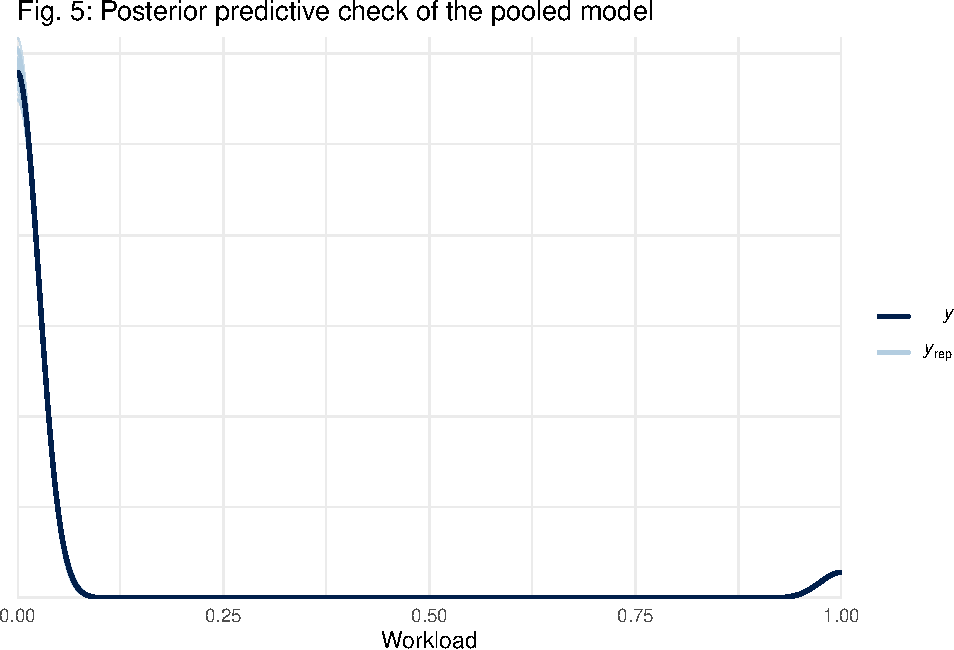
\includegraphics{dissents_article_appendix_files/figure-latex/pp_check_workload-1.pdf}
\vspace{25pt}

We now compare the pooled against the hierarchical models. Both models
got almost indistinguishably similar results. Thus, because the
hierarchical model is computationally more expensive, we opted for the
pooled model.

\begin{longtable}[]{@{}lrrrr@{}}
\caption{Posterior prediction summaries of performance of Model
2}\tabularnewline
\toprule\noalign{}
model & mae & mae\_scaled & within\_50 & within\_95 \\
\midrule\noalign{}
\endfirsthead
\toprule\noalign{}
model & mae & mae\_scaled & within\_50 & within\_95 \\
\midrule\noalign{}
\endhead
\bottomrule\noalign{}
\endlastfoot
hierarchical & 0.05 & 0.22 & 0.95 & 1 \\
pooled & 0.05 & 0.22 & 0.95 & 1 \\
\end{longtable}

\hypertarget{model-3-diagnosis}{%
\subsection{Model 3 diagnosis}\label{model-3-diagnosis}}

Our third model includes a count as a variable of interest. More
specifically, our outcome of interest is the number of dissenting
opinions that a judge wrote in any given year. We thus assume that

\[
Y_{dissents\:count} | \lambda \sim Pois(\lambda)
\] Because this time, we have a time series data and because there are
clusters in the form of the judges themselves, we tested both the
hierarchical and pooled model. The hierarchical model was clustered
around the dissenting judge. The hierarchical model yielded more
accurate results, thus, we opted for the hierarchical model at the cost
of higher computational costs.

\begin{longtable}[]{@{}lrrrr@{}}
\caption{Posterior prediction summaries of performance of Model
3}\tabularnewline
\toprule\noalign{}
model & mae & mae\_scaled & within\_50 & within\_95 \\
\midrule\noalign{}
\endfirsthead
\toprule\noalign{}
model & mae & mae\_scaled & within\_50 & within\_95 \\
\midrule\noalign{}
\endhead
\bottomrule\noalign{}
\endlastfoot
hierarchical\_term & 0.93 & 0.58 & 0.82 & 0.98 \\
pooled\_term & 1.39 & 0.85 & 0.64 & 0.96 \\
\end{longtable}

We ran the third model via Stan with 4 Monte Carlo Markov Chains (MCMC)
of 20000 iterations each, the first 10000 warm up iterations being
discarded. We did diagnosis of all the models. The trace plots reveal
that the chains were stable and probed plausible parameter values, the
density plots of the MCMC show that all 4 chains exhibited similar
behavior, and the autocorrelation between the iterations always dropped
quickly and that the chains were moving around the potential parameter
values quickly.

The posterior predictive check (Fig. 6) reveals that our posterior model
could have done a slightly better job, despite that we couldn't find a
better constelation.

\vspace{25pt}

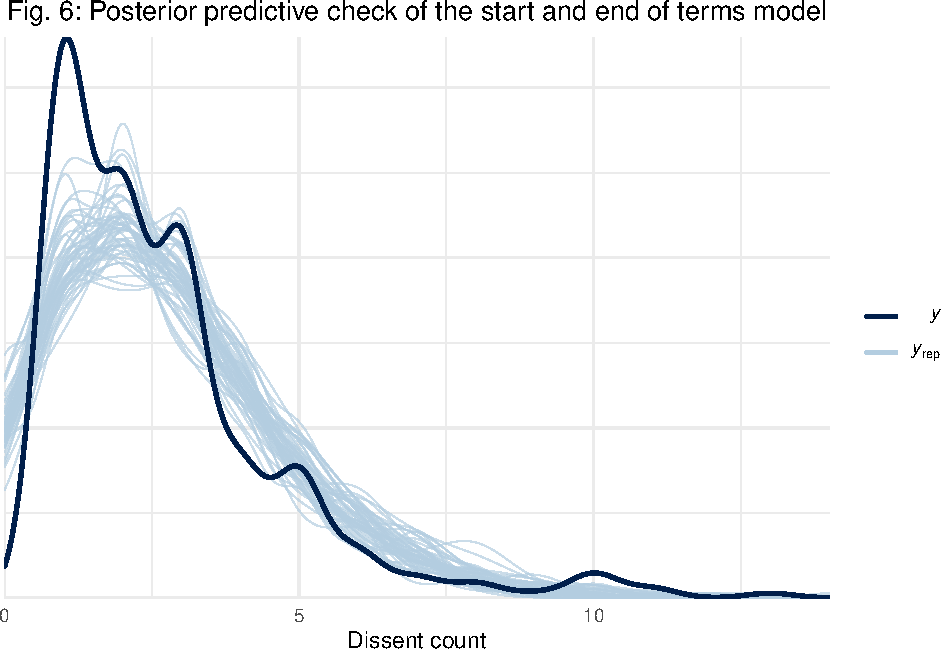
\includegraphics{dissents_article_appendix_files/figure-latex/posterior_check_term-1.pdf}
\vspace{25pt} The diagnostic plots (Fig. 7) also look as they should:
the trace plots show that the chains were stable and probed plausible
parameter values, the density plots of the MCMC show that all 4 chains
exhibited similar behavior, and the autocorrelation between the
iterations always dropped quickly and that the chains were moving around
the potential parameter values quickly.

\vspace{25pt}

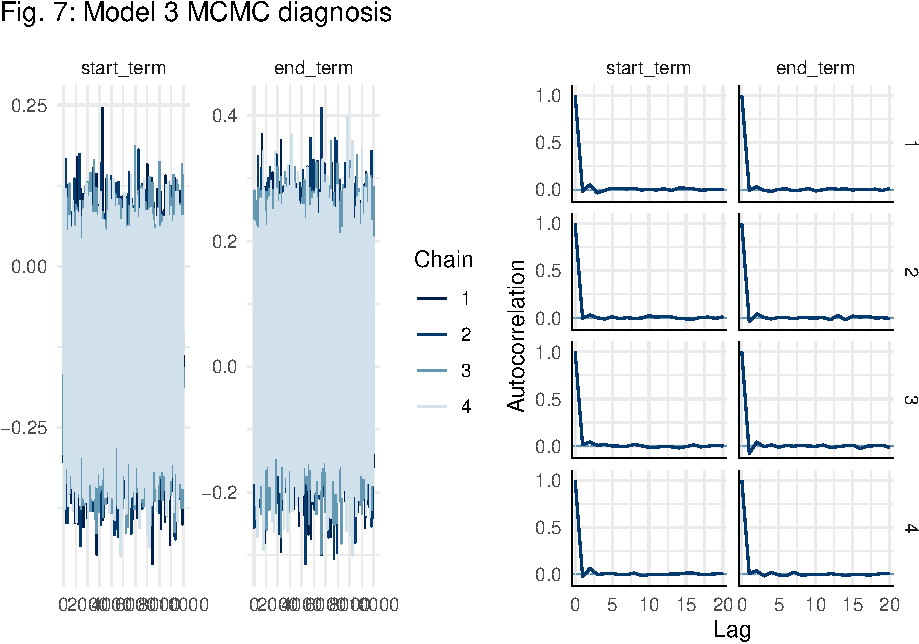
\includegraphics{dissents_article_appendix_files/figure-latex/mcmc_diagnosis_term-1.pdf}
\vspace{25pt}

\hypertarget{model-4-diagnosis}{%
\subsection{Model 4 diagnosis}\label{model-4-diagnosis}}

The outcome variable of interest of our fourth model, the probability of
a judge dissenting in any given decision, is a binomial variable, i.e.,
a Bernoulli distributed variable with 1 trial. The outcome variable thus
follows:

\[ 
Y_{dissent} | \pi \sim Bern(\pi)
\] There were no clusters, thus, we went for a completely pooled model.
As before, because we have zero prior information on the parameters, we
went with weakly uninformative priors. Regarding the diagnosis of the
MCMC chains, the trace plots show that the chains were stable and probed
plausible parameter values, the density plots of the MCMC show that all
4 chains exhibited similar behavior, and the autocorrelation between the
iterations always dropped reasonably quickly, although it could've been
slightly quicker, and that the chains were moving around the potential
parameter values quickly, with the exception of the full\_coalition\_2
parameter, the explanation of which is down to very few data points.

\vspace{25pt}

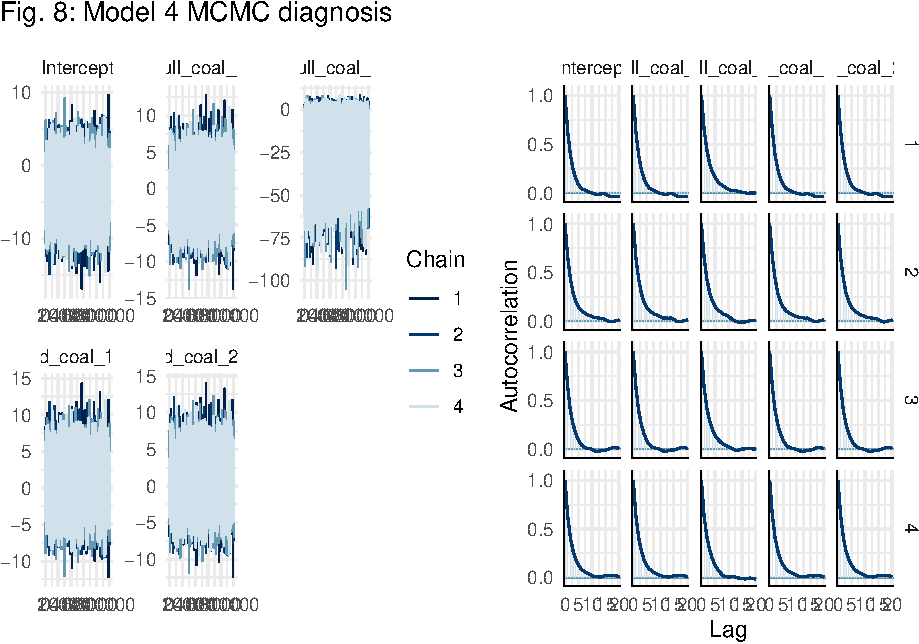
\includegraphics{dissents_article_appendix_files/figure-latex/mcmc_diagnosis_coalition-1.pdf}
\vspace{25pt} Despite that, the posterior predictive check reveals that
our posterior model did a very good job.

\vspace{25pt}

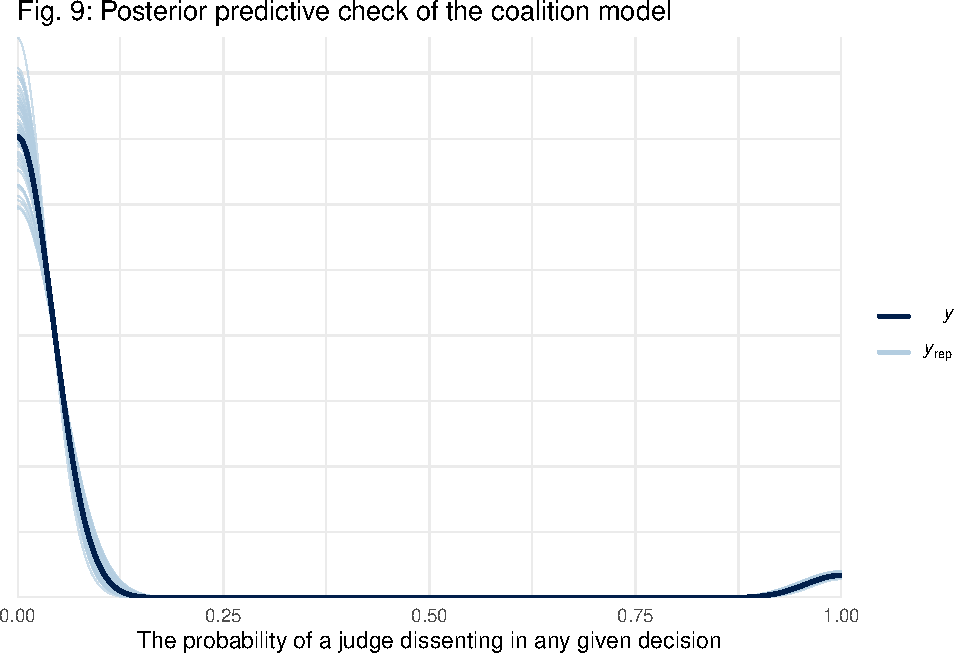
\includegraphics{dissents_article_appendix_files/figure-latex/pp_check_coalition-1.pdf}
\vspace{25pt}

Our model yields reasonably accurate prediction of the underlying data,
the posterior predictive median is only 0.26 standard deviation off from
the observed Y value. Vast majority of the observed Y values fall even
within the 50 \% posterior predictive intervals.

\begin{longtable}[]{@{}lrrrr@{}}
\caption{Posterior prediction summaries of performance of Model
4}\tabularnewline
\toprule\noalign{}
model & mae & mae\_scaled & within\_50 & within\_95 \\
\midrule\noalign{}
\endfirsthead
\toprule\noalign{}
model & mae & mae\_scaled & within\_50 & within\_95 \\
\midrule\noalign{}
\endhead
\bottomrule\noalign{}
\endlastfoot
pooled\_coalition & 0.06 & 0.26 & 0.95 & 0.99 \\
\end{longtable}

\vspace{25pt}

\hypertarget{literature}{%
\section*{Literature}\label{literature}}
\addcontentsline{toc}{section}{Literature}

\hypertarget{refs}{}
\begin{CSLReferences}{1}{0}
\leavevmode\vadjust pre{\hypertarget{ref-eliasekAutomatickaKlasifikaceVyznamovych2020}{}}%
Eliášek, Martin, Jakub Kól, and Miloš Švaňa. 2020. {``Automatická
Klasifikace Významových Celků v Judikatuře.''} \emph{Revue Pro Právo a
Technologie} 11 (21): 3--20. \url{https://doi.org/10.5817/RPT2020-1-1}.

\leavevmode\vadjust pre{\hypertarget{ref-ludersProportionalityArgumentIdentification2023}{}}%
Lüders, Kilian, and Bent Stohlman. 2023. {``Proportionality as an
Argument: {Identification} of a Judicial Decision Technique.''}
\emph{DRAFT for 5th ANNUAL COMPTEXT Conference}.

\leavevmode\vadjust pre{\hypertarget{ref-mikolovEfficientEstimationWord2013}{}}%
Mikolov, Tomas, Kai Chen, Greg Corrado, and Jeffrey Dean. 2013.
{``Efficient {Estimation} of {Word Representations} in {Vector
Space}.''} September 6, 2013.
\url{https://doi.org/10.48550/arXiv.1301.3781}.

\end{CSLReferences}

\end{document}
